\section{Historia}

\begin{frame}[t,shrink=10]{¿De donde viene?}
\begin{columns}[T]

\pause
\column{.5\textwidth}
\begin{block}{Lenguajes de alto nivel}
    \begin{itemize}
      \item Lenguajes de abstracción de propósito general.
        \begin{itemize}
          \item Simula.
        \end{itemize}
      \item Lenguajes de abstración de dominio específico.
        \begin{itemize}
          \item FORTRAN, COBOL.
        \end{itemize}
    \end{itemize}
\end{block}

\pause
\column{.5\textwidth}
\begin{block}{Influencias de bajo nivel}
    \begin{itemize}
      \item Correspondencia directa con el hardware.
        \begin{itemize}
          \item Ensamblador.
        \end{itemize}
      \item Abstracción mínima del hardware.
        \begin{itemize}
          \item BCPL.
          \item C.
        \end{itemize}
    \end{itemize}
\end{block}

\end{columns}

\vfill\pause
\begin{block}{Influencia sobre otros lenguajes}
    \begin{itemize}
      \item Java.
      \item C\#.
      \item C (C11).
    \end{itemize}
\end{block}

\end{frame}


\begin{frame}{Evolución}
\vspace{-0.5em}
\begin{itemize}
  \item Serie de normas ISO/IEC 14882 (1998, 2011, 2014, 2017, 2020, 2023, \ldots).
  \mode<presentation>{\vfill\pause}
  \item \textmark{``Un lenguaje de programación de abstracciones ligeras''} (B. Stroustroup).
  \mode<presentation>{\vfill\pause}
  \item Evolución de C++.
    \begin{itemize}
      \item Tiene muchos elementos de compatibilidad (incluso hasta 1972).
      \item Evolucionar un lenguaje con miles de millones de línea de código es
      distinto que diseñar un nuevo lenguaje de programación.
    \end{itemize}
  \mode<presentation>{\vfill\pause}
  \item Si alguien dice que tiene un lenguaje de programación perfecto:
    \begin{itemize}
      \item Es na\"{i}ve.
      \item Es un vendedor.
    \end{itemize}
\end{itemize}
\end{frame}

\begin{frame}[t]{Normalización}
\vspace{-1em}
\begin{columns}[T]

\column{.8\textwidth}
\begin{itemize}
  \item 1998: C++98 $\rightarrow$ ISO/IEC 14882:1998
  \item 2003: C++03 $\rightarrow$ ISO/IEC 14882:2003.
    \begin{itemize}
      \item Technical Corrigendum
    \end{itemize}
  \item 2005: C++ TR1 $\rightarrow$ ISO/IEC TR 19768.
    \begin{itemize}
      \item C++ Library Extensions
    \end{itemize}
  \item 2011: C++11 $\rightarrow$ ISO/IEC 14882:2011.
  \item 2014: C++14 $\rightarrow$ ISO/IEC 14882:2014. 
  \item 2017: ISO/IEC 14882:2017.
  \item 2020: ISO/IEC 14882:2020.
  \item 2023: ISO/IEC 14882:2023.
  \item 2026: \textbad{???}
\end{itemize}

\column{.2\textwidth}

\includegraphics[width=.8\textwidth]{logos/iso.png}
\end{columns}

\end{frame}

\begin{frame}{ISO C++ a lo largo del tiempo}
\centering
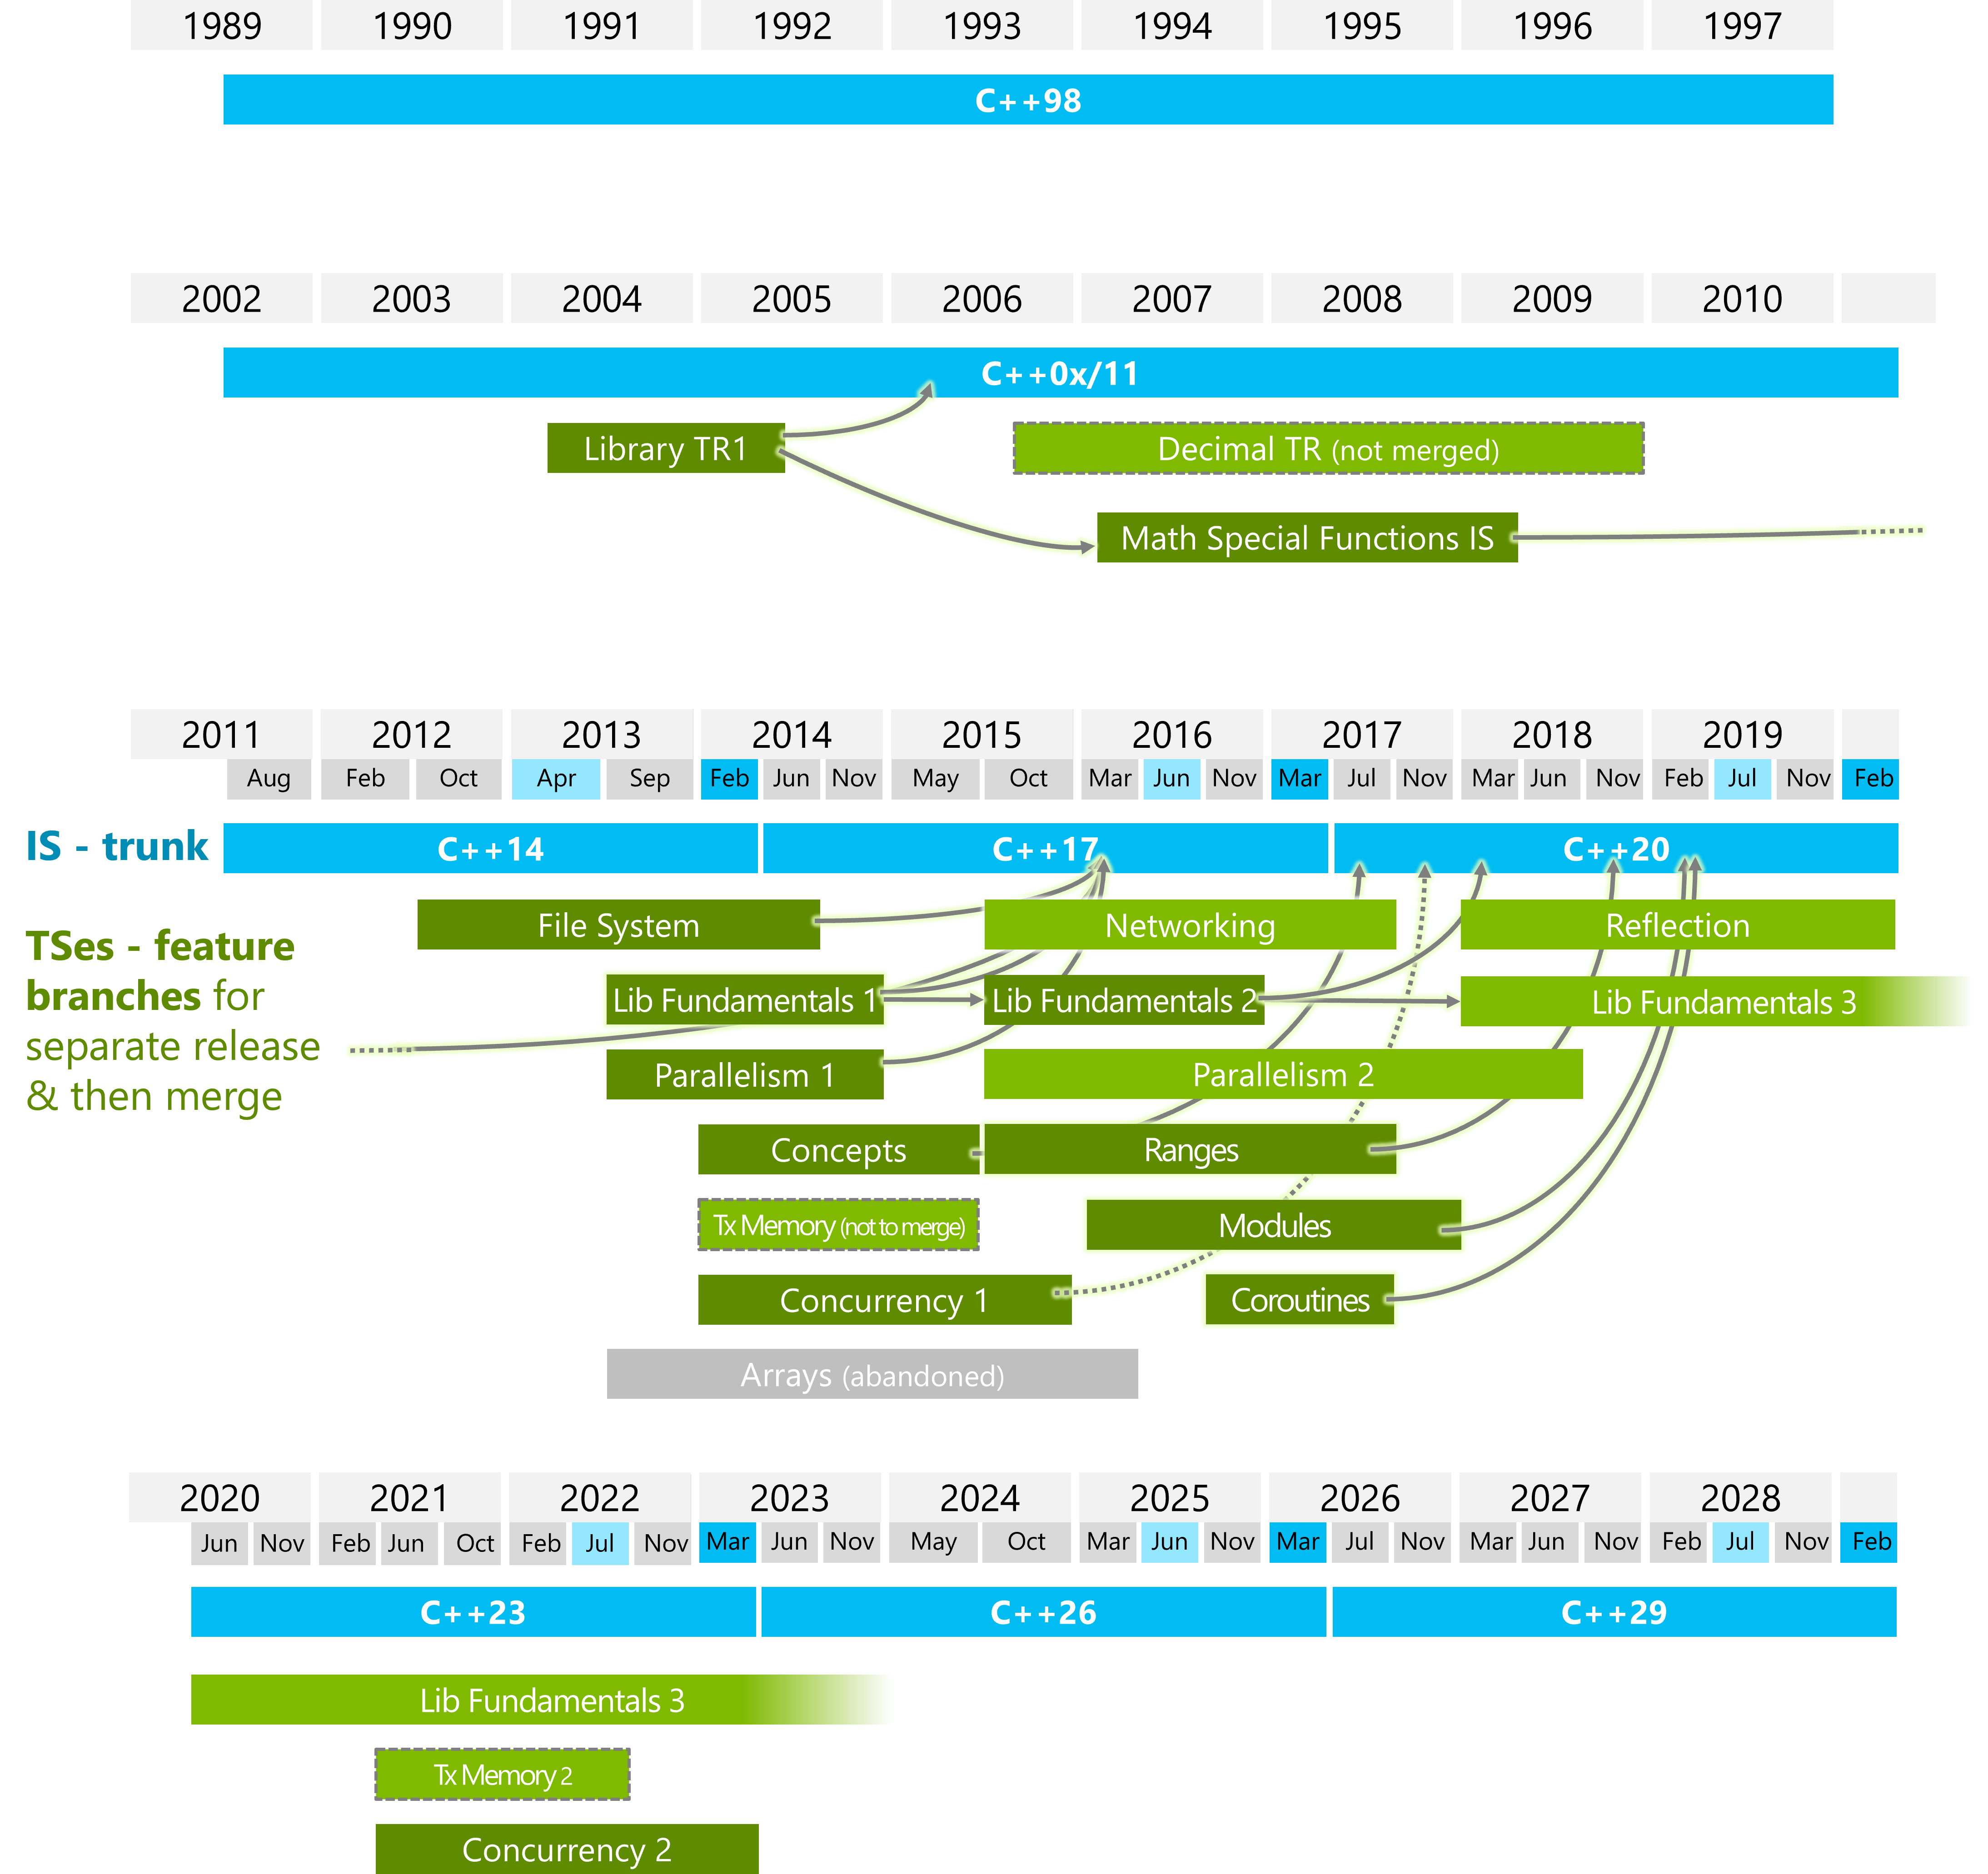
\includegraphics[height=.8\textheight]{img/wg21-timeline-2023.png}
\end{frame}

\begin{frame}[t]{Principios de diseño}
\begin{itemize}
  \item \pause  Mantener compatibilidad hacia atrás.
  \item \pause  Mejor extender la biblioteca que el lenguaje.
  \item \pause  Facilitar el diseño de sistemas y bibliotecas (en vez de dominios concretos).
  \item \pause  Mejorar la seguridad de tipos.
  \item \pause  Mejorar el rendimiento y la interacción con el hardware.
  \item \pause  Principio de \emph{zero-overhead}.
  \item \pause  Hacer C++ más fácil de enseñar y aprender.
\end{itemize}
\end{frame}

\begin{frame}[t]{El comité de C++}
\vspace{-.75em}
\noindent
\centering
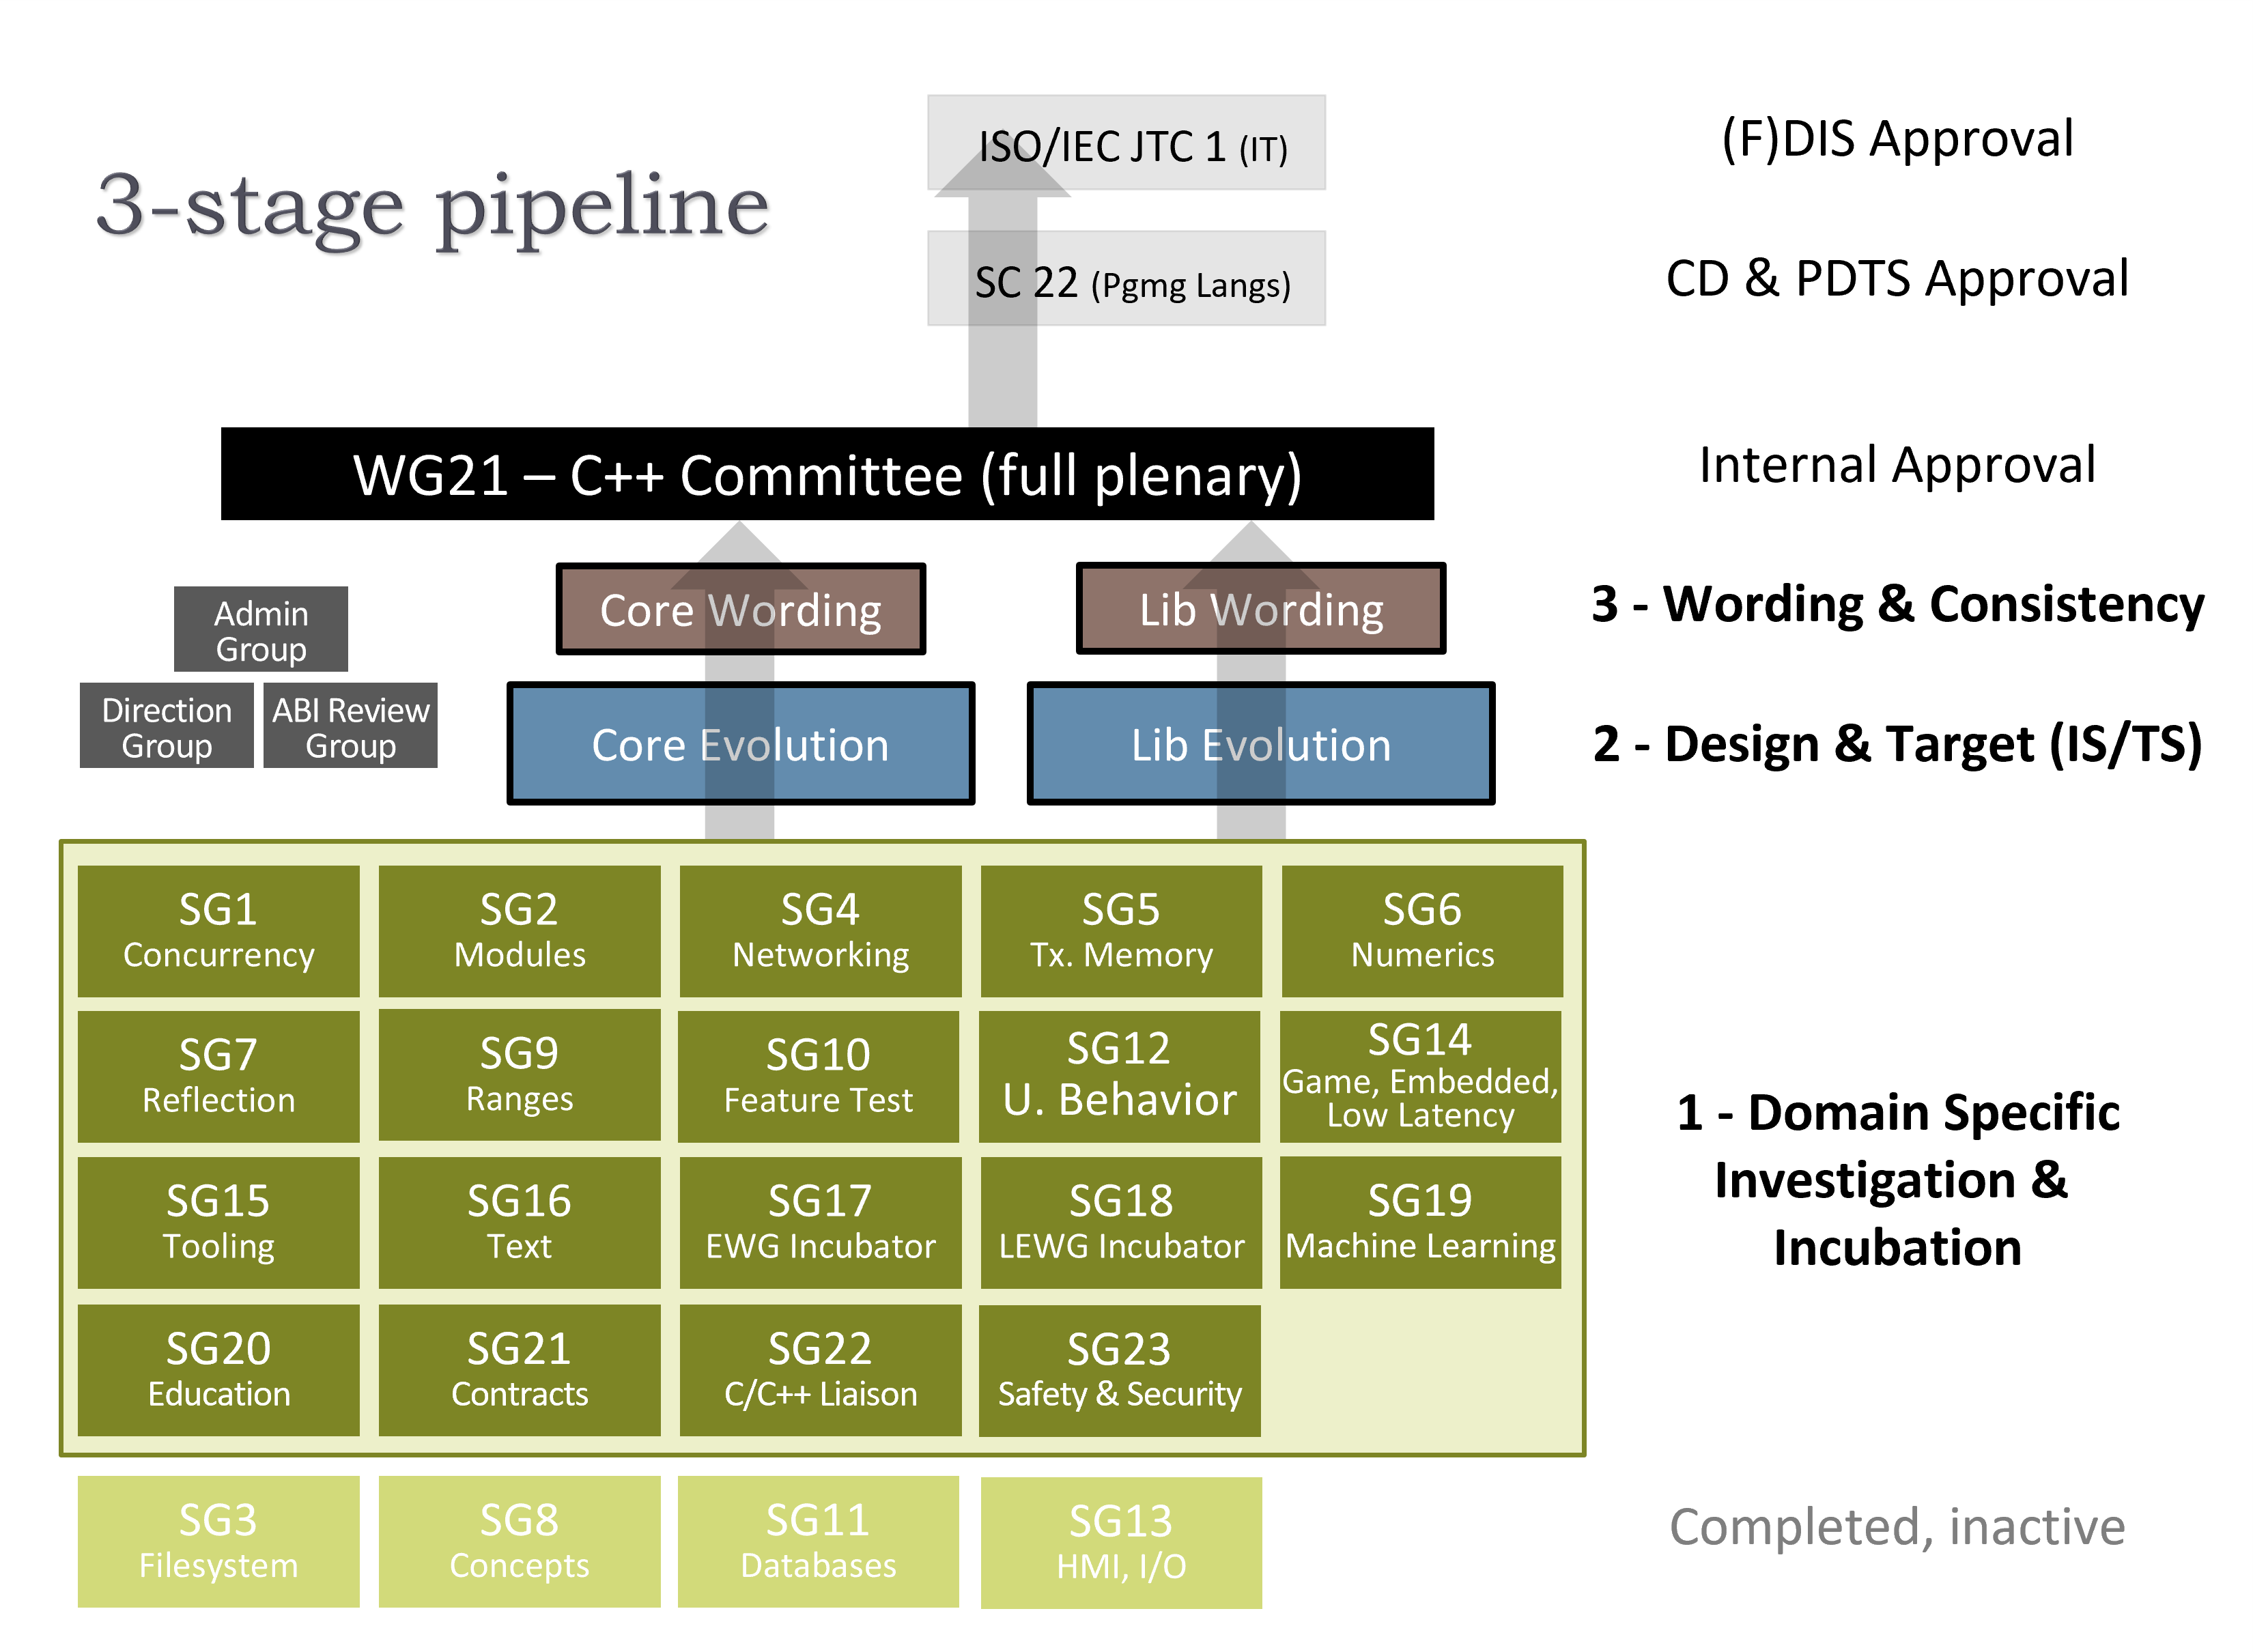
\includegraphics[height=.9\textheight]{img/wg21-structure-2022.png}
\end{frame}

\begin{frame}[t]{¿Cuanta gente participa?}
\vspace{-1em}
\begin{columns}
\column{.7\textwidth}
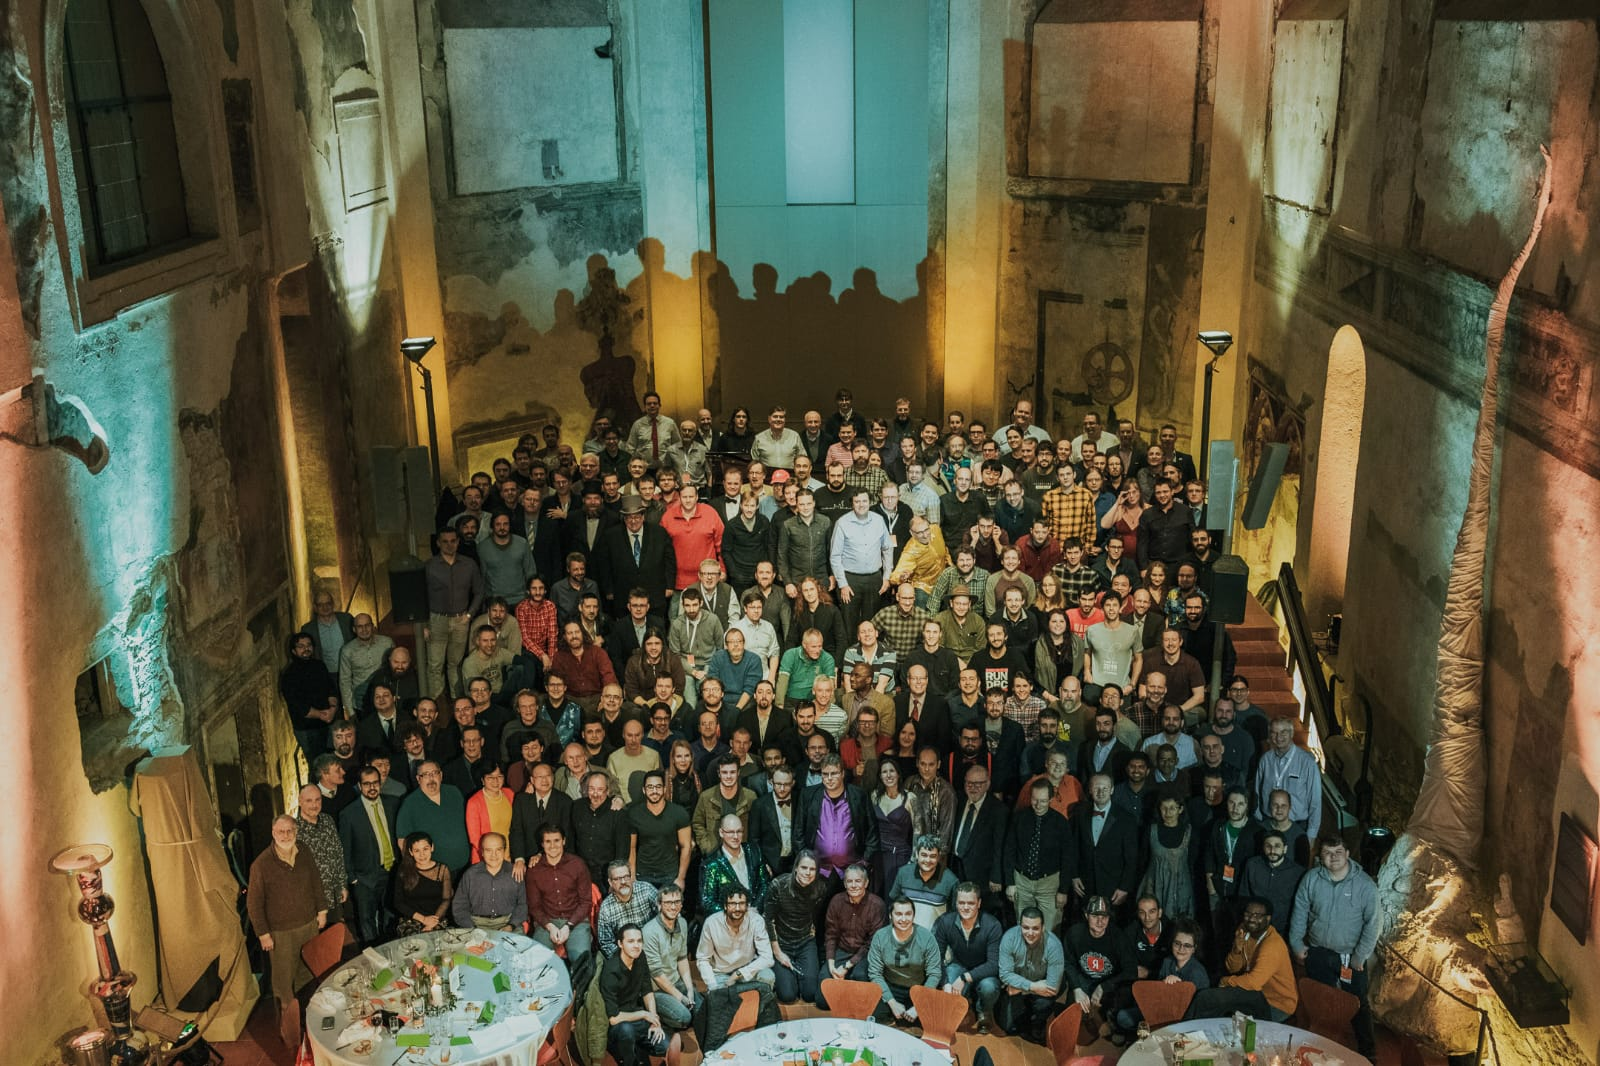
\includegraphics[height=.9\textheight]{img/full-committee-prague.jpg}
\column{.3\textwidth}

\includegraphics[width=1em]{img/flags/at.jpg}

\includegraphics[width=1em]{img/flags/bg.jpg}

\includegraphics[width=1em]{img/flags/ca.jpg}

\includegraphics[width=1em]{img/flags/cn.jpg}
\\

\includegraphics[width=1em]{img/flags/cz.jpg}

\includegraphics[width=1em]{img/flags/dk.jpg}

\includegraphics[width=1em]{img/flags/fi.jpg}

\includegraphics[width=1em]{img/flags/fr.jpg}
\\

\includegraphics[width=1em]{img/flags/de.jpg}

\includegraphics[width=1em]{img/flags/ie.jpg}

\includegraphics[width=1em]{img/flags/il.jpg}

\includegraphics[width=1em]{img/flags/it.jpg}
\\

\includegraphics[width=1em]{img/flags/jp.jpg}

\includegraphics[width=1em]{img/flags/kr.jpg}

\includegraphics[width=1em]{img/flags/nl.jpg}

\includegraphics[width=1em]{img/flags/no.jpg}
\\

\includegraphics[width=1em]{img/flags/pl.jpg}

\includegraphics[width=1em]{img/flags/pt.jpg}

\includegraphics[width=1em]{img/flags/ro.jpg}

\includegraphics[width=1em]{img/flags/ru.jpg}
\\

\includegraphics[width=1em]{img/flags/sk.jpg}

\includegraphics[width=1em]{img/flags/es.jpg}

\includegraphics[width=1em]{img/flags/ch.jpg}

\includegraphics[width=1em]{img/flags/se.jpg}
\\

\includegraphics[width=1em]{img/flags/gb.jpg}

\includegraphics[width=1em]{img/flags/us.jpg}
\end{columns}
\end{frame}
